\chapter{Introduction}
\label{sec:intro}
\textbf{TODO}
\begin{itemize}
	\item{Explain Context in which SHAMPU was designed}
	\item{Explain Problem SHAMPU tries to fix}
	\item{Explain "Problem" of this thesis "ANT as an addition to SHAMPU, need to know how good ANT is"}
	\item{Explain how problem was solved, e.g. Different experiments which try to evaluate ANT in the context of SHAMPU}
\end{itemize}
In this thesis we evaluate the WSN testbed: SHAMPU (Single chip Host for Autonomous Mote Programming over USB). 


\section{Related work}
\label{sec:related_work}

There are already several different WSN testbeds available. These testbeds all fulfil certain roles, but ultimately fail to provide all the necessary features for a small, mobiles and low power WSN testbed.\\

There are some testbeds which need a fixed infrastructure, like FlockLab \cite{Lim2013} or Minverva \cite{Sommer}. The nature of a fixed infrastructure has certain problems. For once it might only be  viable to test inside the lab and not in the target environment since the needed infrastructure is often only available inside a lab or not easily transportable. 

Other technologies aim to detach the testbed from the infrastructure itself and rely on wireless communication instead. Sensei-UU \cite{Rensfelt2009} for example uses a wireless 802.11 network for communication between the nodes and the sensor host. The problem here is the power requirements for the communication, which makes it hard to run the nodes without an external power source.

BTNodes \cite{Moser} or Smart-Its \cite{Kasten2000} use Bluetooth to address the power issue. But Bluetooth introduces different problems, such as size limitations for the network and a difficult set-up and use of more complex network topologies. The newest version of Bluetooth tries to address this with the introduction of ScatterNets, but the setup and maintenance of the network still remains challenging.

\chapter{Technical Background}
\section{SHAMPU}
SHAMPU (Single chip Host for Autonomous Mote Programming over USB) \cite{Smeets:2014:DAL:2602339.2602401} is a WSN testbed, which allows the remote debugging and reprogramming of sensor nodes. The main advantages over other testbeds (see section~\ref{sec:related_work}) are the low cost, small size and low energy consumption. SHAMPU can be used as an extension to an already existing sensor node. The node only needs to provide an USB-Interface, SHAMPU is thus completely OS independent.
\begin{figure}[h]
\centering
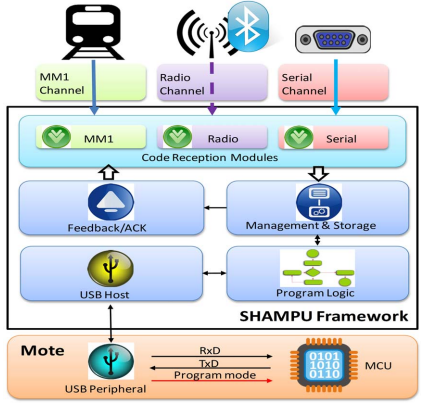
\includegraphics[scale=.5]{./pics/SHAMPUframework.png}
\caption{Overview of the SHAMPU Framework}\label{fig:shampuframework}
\end{figure}
The SHAMPU framework (see Figure \ref{fig:shampuframework}) itself is split into multiple modules. The Code Reception Module allows the use of different protocols to connect to and communicate with other SHAMPU enabled devices. For wireless communication SHAMPU uses an ANTAP1MxIB RF Transceiver Module, which supports the ANT protocol. The USB Host module is used to connect to the sensor node, which SHAMPU is attached to.

\section{ANT}
ANT \cite{DynastreamInnovationsInc.2013} is a wireless protocol which operates in the 2.4 GHz ISM Band. Originally developed in 2003 by Dynastream Innovations Inc. for the use wireless sensors. The ANT protocol is designed for the use in low power WSNs and puts a focus on scalability and ease of use.
\begin{figure}[h]
\centering
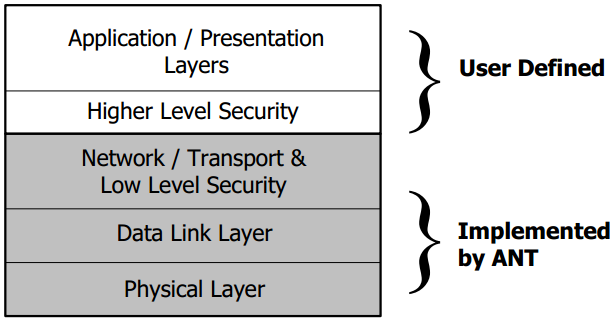
\includegraphics[scale=.5]{./pics/ANTstack.png}
\caption{OSI-Layer vs. ANT Protocol}\label{fig:osilayer}
\end{figure}
One of the advantages ANT has over other protocols, like Bluetooth or ZigBee is the high level of abstraction the ANT Protocol provides. This is achieved by the incorporation the first 4 OSI-layer (see Figure \ref{fig:osilayer}) into the ANT protocol and thus allowing even low-cost MCU to setup and maintain complex wireless networks.

\subsection{ANT Topology}
In order for the ANT protocol to work each mote needs to be part of a network. As shown in figure \ref{fig:anttopo} the ANT protocol can be used to create simple or more complex networks. Each mote inside a network is called an ANT node and in order for two nodes to communicate with each other they need to be connected via a channel.

\begin{figure}[h]
	\centering
	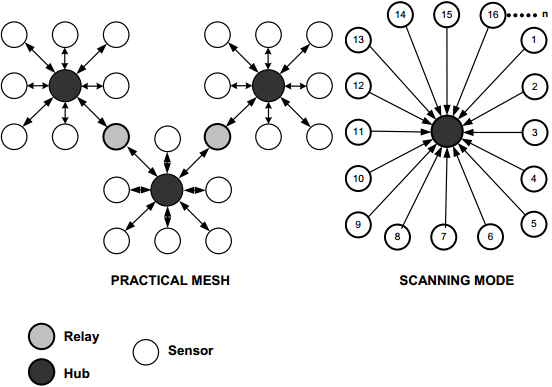
\includegraphics[scale=0.7]{./pics/ANTtopo.png}
	\caption{Example ANT Topologies}\label{fig:anttopo}
\end{figure}


\subsection{ANT Channels}
Most of the available channel types are bidirectional, but the ANT protocol still differentiates between master and slaves nodes. While a master nodes mostly sends data and a slave nodes mostly receives data, the slave still has the ability to response to the incoming data.

The ANT protocol knows 125 different channels, each 1 MHz wide. Each Channel supports a data rate of 1 Mbps and up to 65533 nodes. To avoid interference between the channels isochronous self adjusting TDMA technology is used, this allows the ANT nodes to change the transmit timings and even the frequency that is being used for the current channel.

\textit{Picture Process to establish a channel between master and slave nodes.}

The ANT protocol distinguishes between 2 different Channel types:
\begin{description}
\item{\textbf{Independent Channels}} \hfill \\ Independent Channels are used if there is only one node, which is transmitting data. There is no limit of the amount of slave devices, which receive the messages being send out. Furthermore the message being send out is broadcast to all nodes, it is not possible to only address a specific node.
\item{\textbf{Shared Channels}} \hfill \\ Shared Channels are used if a single ANT node needs to receive data from many nodes. This type of channel is made possible by the use of Shared Channel Address, however this reduces the amount of data that can be transmitted at a time. The Channel master can decided to either use one or two bytes as the address, which allows for either 255 or 65535 slave devices in the same channel.
\end{description}

\subsection{ANT Communication}
The ANT protocol supports 4 different data types: broadcast, acknowledge, burst and advanced burst. The data type is not part of the channel configuration and thus channels are able to use any combination of data types. The only exceptions are unidirectional channels, which can only ever send broadcast data.
\begin{itemize}
	\item{Broadcast data} \hfill \\ Broadcast data is the most basic datatype and the default choice since it uses the least amount of power and bandwidth. Broadcast data is send every timeslot, and if no new data needs to be transmitted, the last send packet is repeated event if it wasn't broadcast in the first place.
	\item{Acknowledge data} \hfill \\ Acknowledge data can only be used in bidirectional channels. Whenever a node receives an acknowledge data packet it immediately sends an acknowledge message back to the sender of original packet to confirm the correct transmission of the data.  
	\item{Burst data} \hfill \\ Burst data provides a method to transmit large amounts of data. This is achieved by ignoring the normal channel period and sending the packets right after each other. This allows for a transmission rate of upto 20 kbps, much higher than other data transmissions types. There is no limit for the duration of the burst, however since burst data takes precedence over all other traffic, care should be taken care to allow other devices to transmit data.
	\item{Advanced burst data} \hfill \\ This type of data is only supported on some ANT devices, it pushed the maximum transmission rate to 60 kbps, but is otherwise the same as normal burst data.
\end{itemize}

\subsection{ANT messages}
In the ANT protocol each message has the in Figure \ref{fig:antmsg} specified basic format.
\begin{figure}[h]
	\centering
	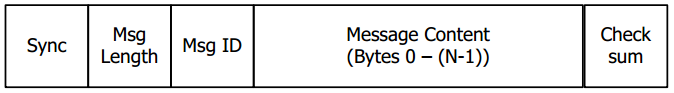
\includegraphics[scale=.75]{./pics/ANTmsg.png}
	\caption{Ant message structure}\label{fig:antmsg}
\end{figure}
Each message starts with a special Sync-Byte and end with a checksum, which is calculated by xoring all previous bytes. The Msg Length byte is the number ob Message Content bytes. The Msg ID byte specifies which kind of data is contained in the message. The ANT protocol also provides an extended message format, which allows to attached further information to each message.


\section{ANTAP1MxIB RF}
In order to use the ANT protocol each SHAMPU-mote is equipped with an ANTAP1MxIB RF Transceiver Module. The module was chosen because of it's small form factor (20mm x 20mm) and very low power draw. The ANTAP1M can handle up to 4 ANT channels and a 1Mbps RF data rate, which is enough to setup and use the desired network topology.

The proposed experiments are run with two different kinds of hardware.

\begin{itemize}
	\item{ANT Basestation} \hfill \\ The Basestation contains the ANT Module and a \textbf{IC-Name} which allows the basestation to be connected via RS-232 to a PC.
	\item{SHAMPU node} \hfill \\ The ANT Module is directly connected to the SHAMPU node in an asyncronous and is used just like any other 
\end{itemize}

\chapter{Evaluation of SHAMPU}
In order to assess the capabilities of SHAMPU we plan and run experiments designed to evaluate the SHAMPU framework in the following three categories:
\begin{itemize}
	\item{\textbf{Communication Range}} 
	\item{\textbf{Communication Delay}} 
	\item{\textbf{Data Throughput}} 
\end{itemize}

For this we designed different scenarios, which test one or more of the described categories. The following section describes the experiments according to the following template:

\begin{description}
\item{\textbf{Description}} \hfill \\ A description of the experiment and the the category being evaluated.
\item{\textbf{Network Topology}} \hfill \\ A diagram of the network topology in which the experiment is run.
\item{\textbf{Testing methodology}} \hfill \\ A description on how the experiment is performed.
\item{\textbf{Result}} \hfill \\ The results of the experiment and any additional collected data.
\end{description}

All the experiments were done on the third floor of the SA building of the University Duisburg-Essen.
\newpage

\section{Experiment 1: Delay calculations between two nodes}
\begin{description} 
	\item{\textbf{Description}} \hfill \\ In this experiment we try to determine the communication delay between two nodes. For this we use a simple ping application. Node A starts by sending a ping packet to Node B. Node B acknowledges the message and response with a ping message of its own. Node A acknowledges that message and repeats the whole process.
	\item{\textbf{Network Topology}} \hfill \\ \textit{Diagram for the experiment:  2 nodes right next to eachother. A node is master, B node is slave.} 
	\item{\textbf{Testing methodology}} \hfill \\ As shown in figure (zzz) the delay of each transmission can be split into two different parts:\\
	$d_1$ Delay Node A $\rightarrow$ Node B + 0 to $\frac{1}{freq}$\\
	$d_2$ Delay Node B $\rightarrow$ Node A + 0 to $\frac{1}{freq}$\\
	$d_3$ Delay PC $\rightarrow$ Node A\\
	$d_4$ Delay PC $\rightarrow$ Node B\\
	\begin{align*}
	d_1 &= D - \frac{C}{2} + \frac{D-C}{2}\\
	d_2 &= B + \frac{C}{2} + \frac{D-C}{2}\\
	d_3 &= \frac{D-C}{2}\\
	d_4 &= \frac{C}{2}\\
	\end{align*}
	1. Prepare Pingpayload [1 Byte == 1 char ‚p‘]\\
	2. Save sendTimestamp in PC and send to Slave\\
	3. Message arrives @ Slave:\\
		3.1 directly reply msg to Master B = clock() – [savedTime]\\
		3.2 msg to PC A = clock() – [savedTime]\\
	4. Prep Pongpayload [1 Byte == 1 char ‚P‘]\\
	5. Save sendTimestamp in PC and send to Master\\
	6. Message arrives @ Master:\\
		6.1 directly reply msg to Slave D = clock() - [savedTime]\\
		6.2 msg to PC C = clock() – [savedTime]\\
	  
	\item{\textbf{Result}} \hfill \\ In Diagram (x) shows the transmission failures for each of the different runs. 
\end{description}

\newpage

\section{Experiment 2: Delay calculations between multiple nodes}
\newpage

\section{Experiment 3: Maximal communication Range}
\begin{description} 
\item{\textbf{Description}} \hfill \\ According to the datasheet the maximum range for communication is 30m. The ANT documentation doesn't specify for which power setting this range can be achieved. Since we try to minimize power use, we run the experiment with different power settings to try to discover the effects the power setting has on the communication range.
\item{\textbf{Network Topology}} \hfill \\ \textit{Diagram for the experiment:  2 nodes   x meter apart.  with distances from 0.5 m to 30m  (floor in SM 3xx is 27m long)  A node is master, B node is slave. Node B is set up on a movable platform.} 
\item{\textbf{Testing methodology}} \hfill \\ At the beginning of the experiment Node A and B are placed right next to each other. Node A acts as a master and keeps broadcasting the same message. Node B is the slave and tries to receive the broadcast message of Node A. After 20 broadcast messages are send, the transmission failures and successes are recorded and the distance between the two nodes is increased by 0.5 meters. This process is repeated until there no more successful transmissions. At this point the distance is no longer increased, but decreased until a successful transmission can be recorded again. The whole experiment is then repeated for each available power setting 
\item{\textbf{Result}} \hfill \\ In Diagram (x) shows the transmission failures for each of the different runs. 
\end{description}
\newpage

\section{Experiment 4: Data Transfer between two nodes}
The ANT protocol promises a speed of up to 1 Mbps, 20 kbps of which are available for the application itself. In this experiment we try to determining the speed with which it is possible to move data to and form a SHAMPU device. We also try to determinate what effect the size of the payload and the number of the nodes in the network have on the transmission speed.
\newpage

\section{Experiment 5: Reflash of a wireless sensor network}

\chapter{Conclusion}
\textbf{TODO}
\section{Summary}
\textbf{TODO}
\section{Future Work}
\textbf{TODO}
